\documentclass[compress,red]{beamer}
\usepackage[utf8]{inputenc}
\usepackage{ucs}
\usepackage{amsmath}
\usepackage{amsfonts}
\usepackage{amssymb}
\usepackage[russian]{babel}
\usepackage{graphicx}
\usepackage{wrapfig}

\usepackage{tikz}
\usepackage{verbatim}

\usepackage{color}
\usepackage{xcolor}
\usepackage{listings}

\usepackage{caption}
\DeclareCaptionFont{white}{\color{white}}
\DeclareCaptionFormat{listing}{\colorbox{gray}{\parbox{\textwidth}{#1#2#3}}}
\captionsetup[lstlisting]{format=listing,labelfont=white,textfont=white}

\usetikzlibrary{calc,trees,positioning,arrows,chains,shapes.geometric,%
    decorations.pathreplacing,decorations.pathmorphing,shapes,%
    matrix,shapes.symbols}

\tikzset{
>=stealth',
  punktchain/.style={
    rectangle, 
    rounded corners, 
    % fill=black!10,
    draw=black, very thick,
    text width=10em, 
    minimum height=3em, 
    text centered, 
    on chain},
  line/.style={draw, thick, <-},
  element/.style={
    tape,
    top color=white,
    bottom color=blue!50!black!60!,
    minimum width=8em,
    draw=blue!40!black!90, very thick,
    text width=10em, 
    minimum height=1.5em, 
    text centered, 
    on chain},
  every join/.style={->, thick,shorten <=1pt},
  decoration={brace},
  tuborg/.style={decorate},
  tubnode/.style={midway, right=2pt},
}

\mode<presentation>

\usetheme{Warsaw}

\definecolor{Red}{rgb}{1,0,0}
\definecolor{Blue}{rgb}{0,0,1}
\definecolor{Green}{rgb}{0,1,0}
\definecolor{magenta}{rgb}{1,0,.6}
\definecolor{lightblue}{rgb}{0,.5,1}
\definecolor{lightpurple}{rgb}{.6,.4,1}
\definecolor{gold}{rgb}{.6,.5,0}
\definecolor{orange}{rgb}{1,0.4,0}
\definecolor{hotpink}{rgb}{1,0,0.5}
\definecolor{newcolor2}{rgb}{.5,.3,.5}
\definecolor{newcolor}{rgb}{0,.3,1}
\definecolor{newcolor3}{rgb}{1,0,.35}
\definecolor{darkgreen1}{rgb}{0, .35, 0}
\definecolor{darkgreen}{rgb}{0, .6, 0}
\definecolor{darkred}{rgb}{.75,0,0}

\xdefinecolor{olive}{cmyk}{0.64,0,0.95,0.4}
\xdefinecolor{purpleish}{cmyk}{0.75,0.75,0,0}

\useoutertheme[subsection=false]{smoothbars}


\title{Моделирование случайных процессов}
\author{Информатика \\ 10-11 классы}

%\usecolortheme{dolphin}


\begin{document}
%%титульная страница
\maketitle
%% основные моменты

\section{Случайные величины}

\subsection{Монте-Карло}
\begin{frame}[fragile]
  \frametitle{Монте-Карло}
  \centerline{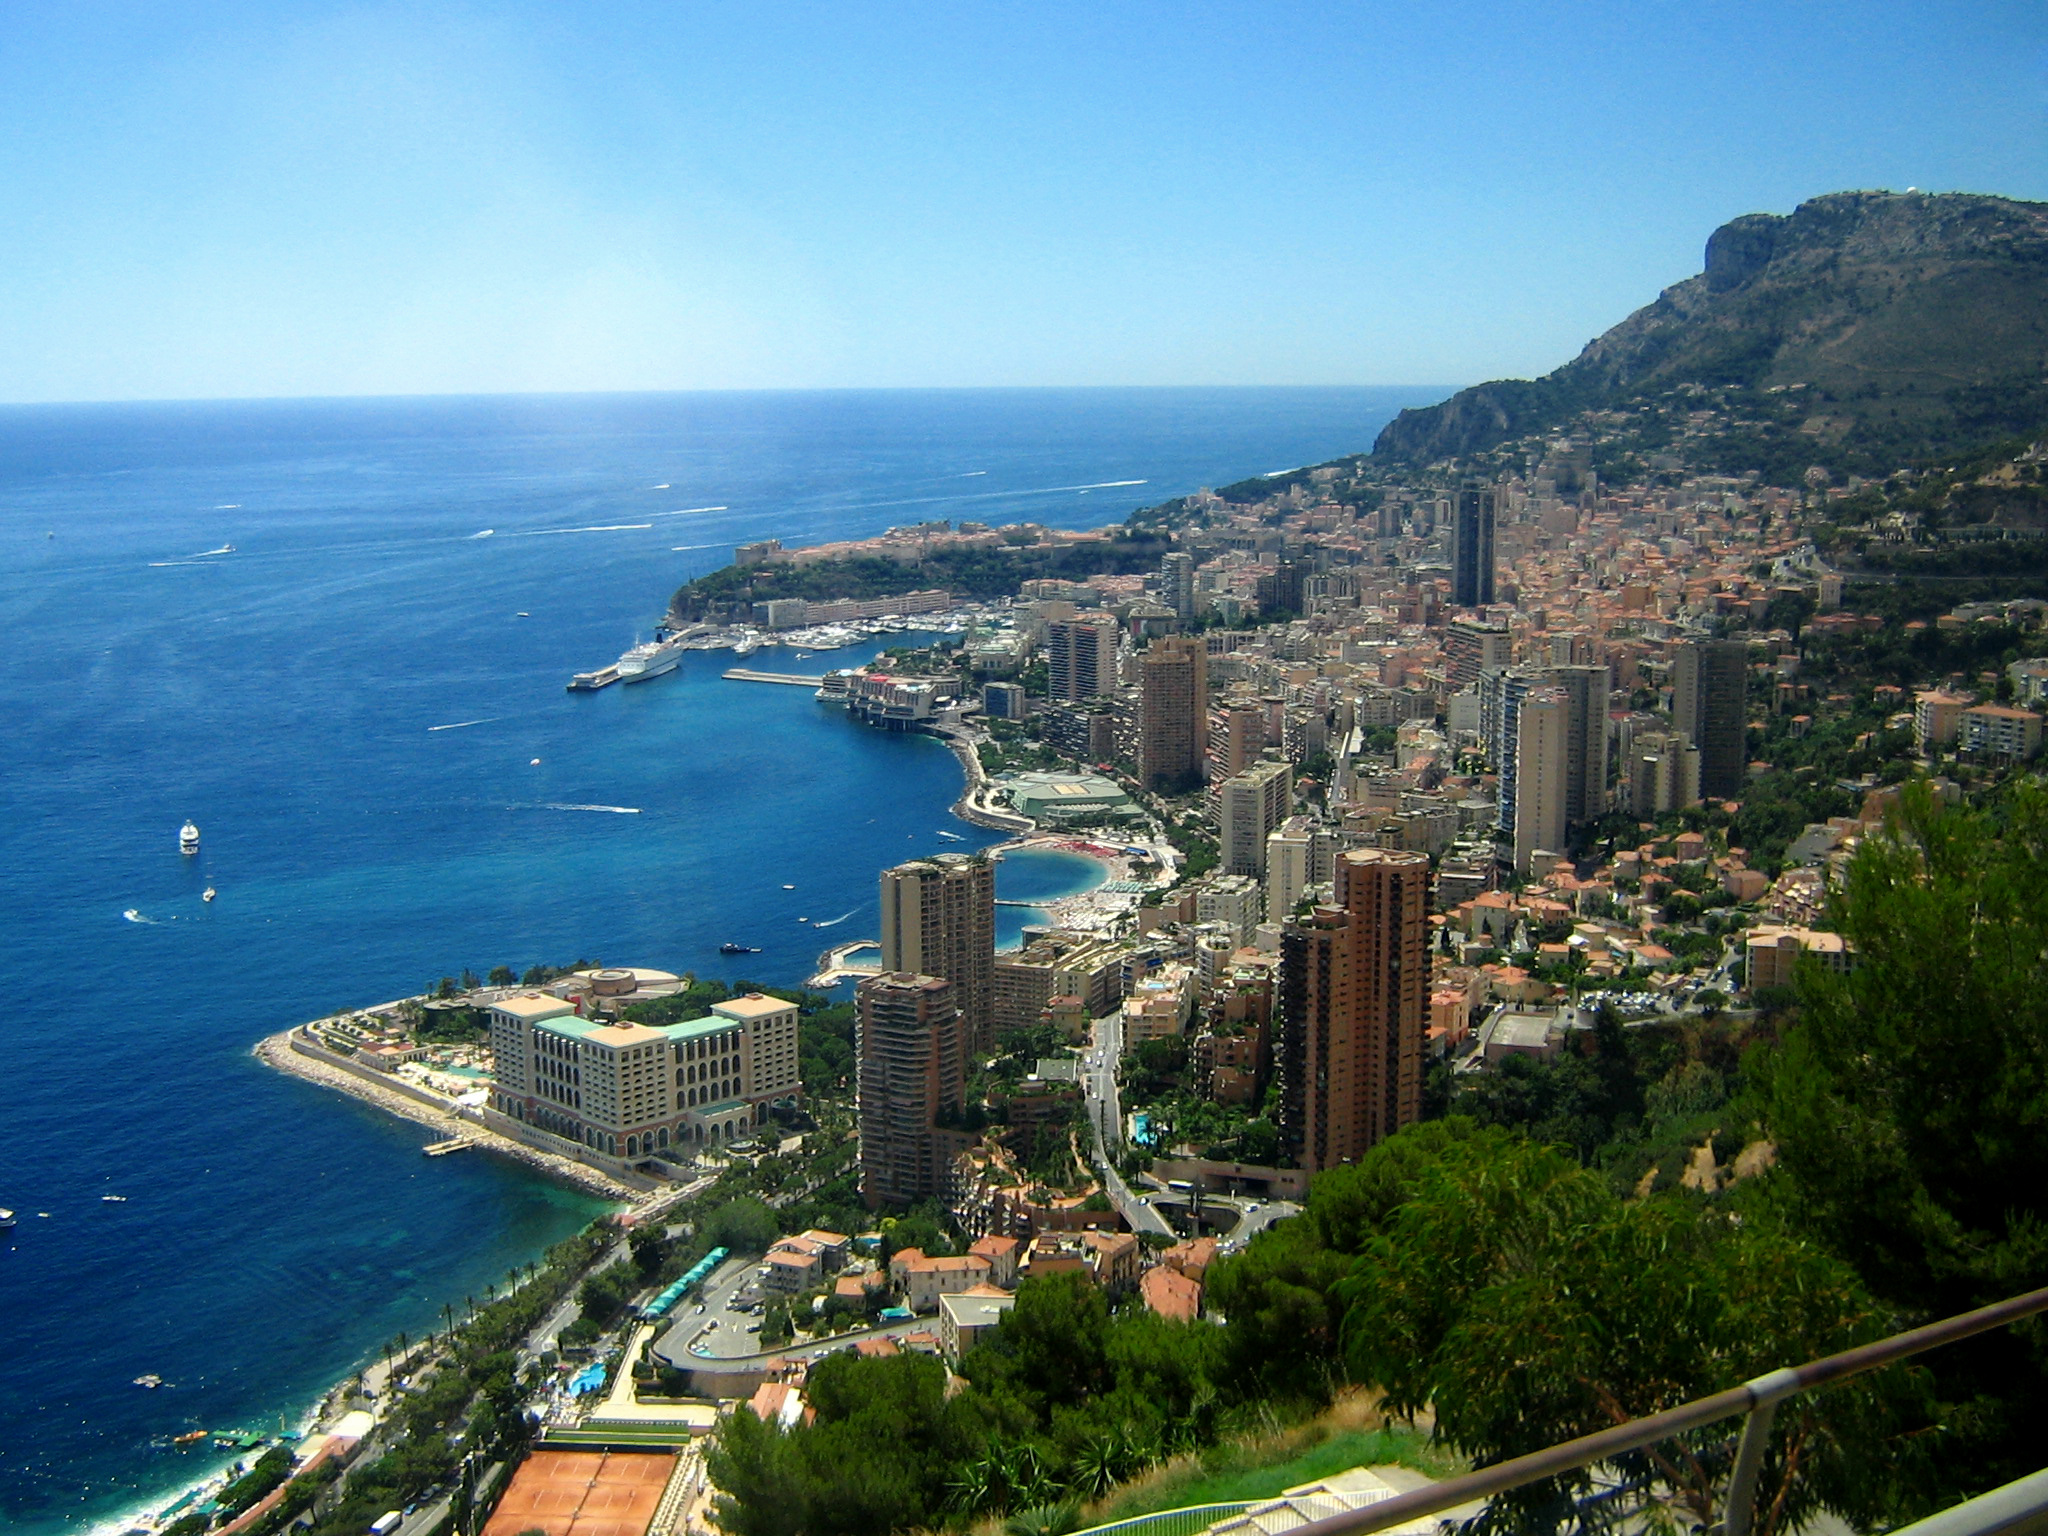
\includegraphics[width=0.7\textwidth]{images/monaco-01.jpg}}
\end{frame}

\subsection{Монте-Карло}
\begin{frame}[fragile]
  \frametitle{Монте-Карло}
  \centerline{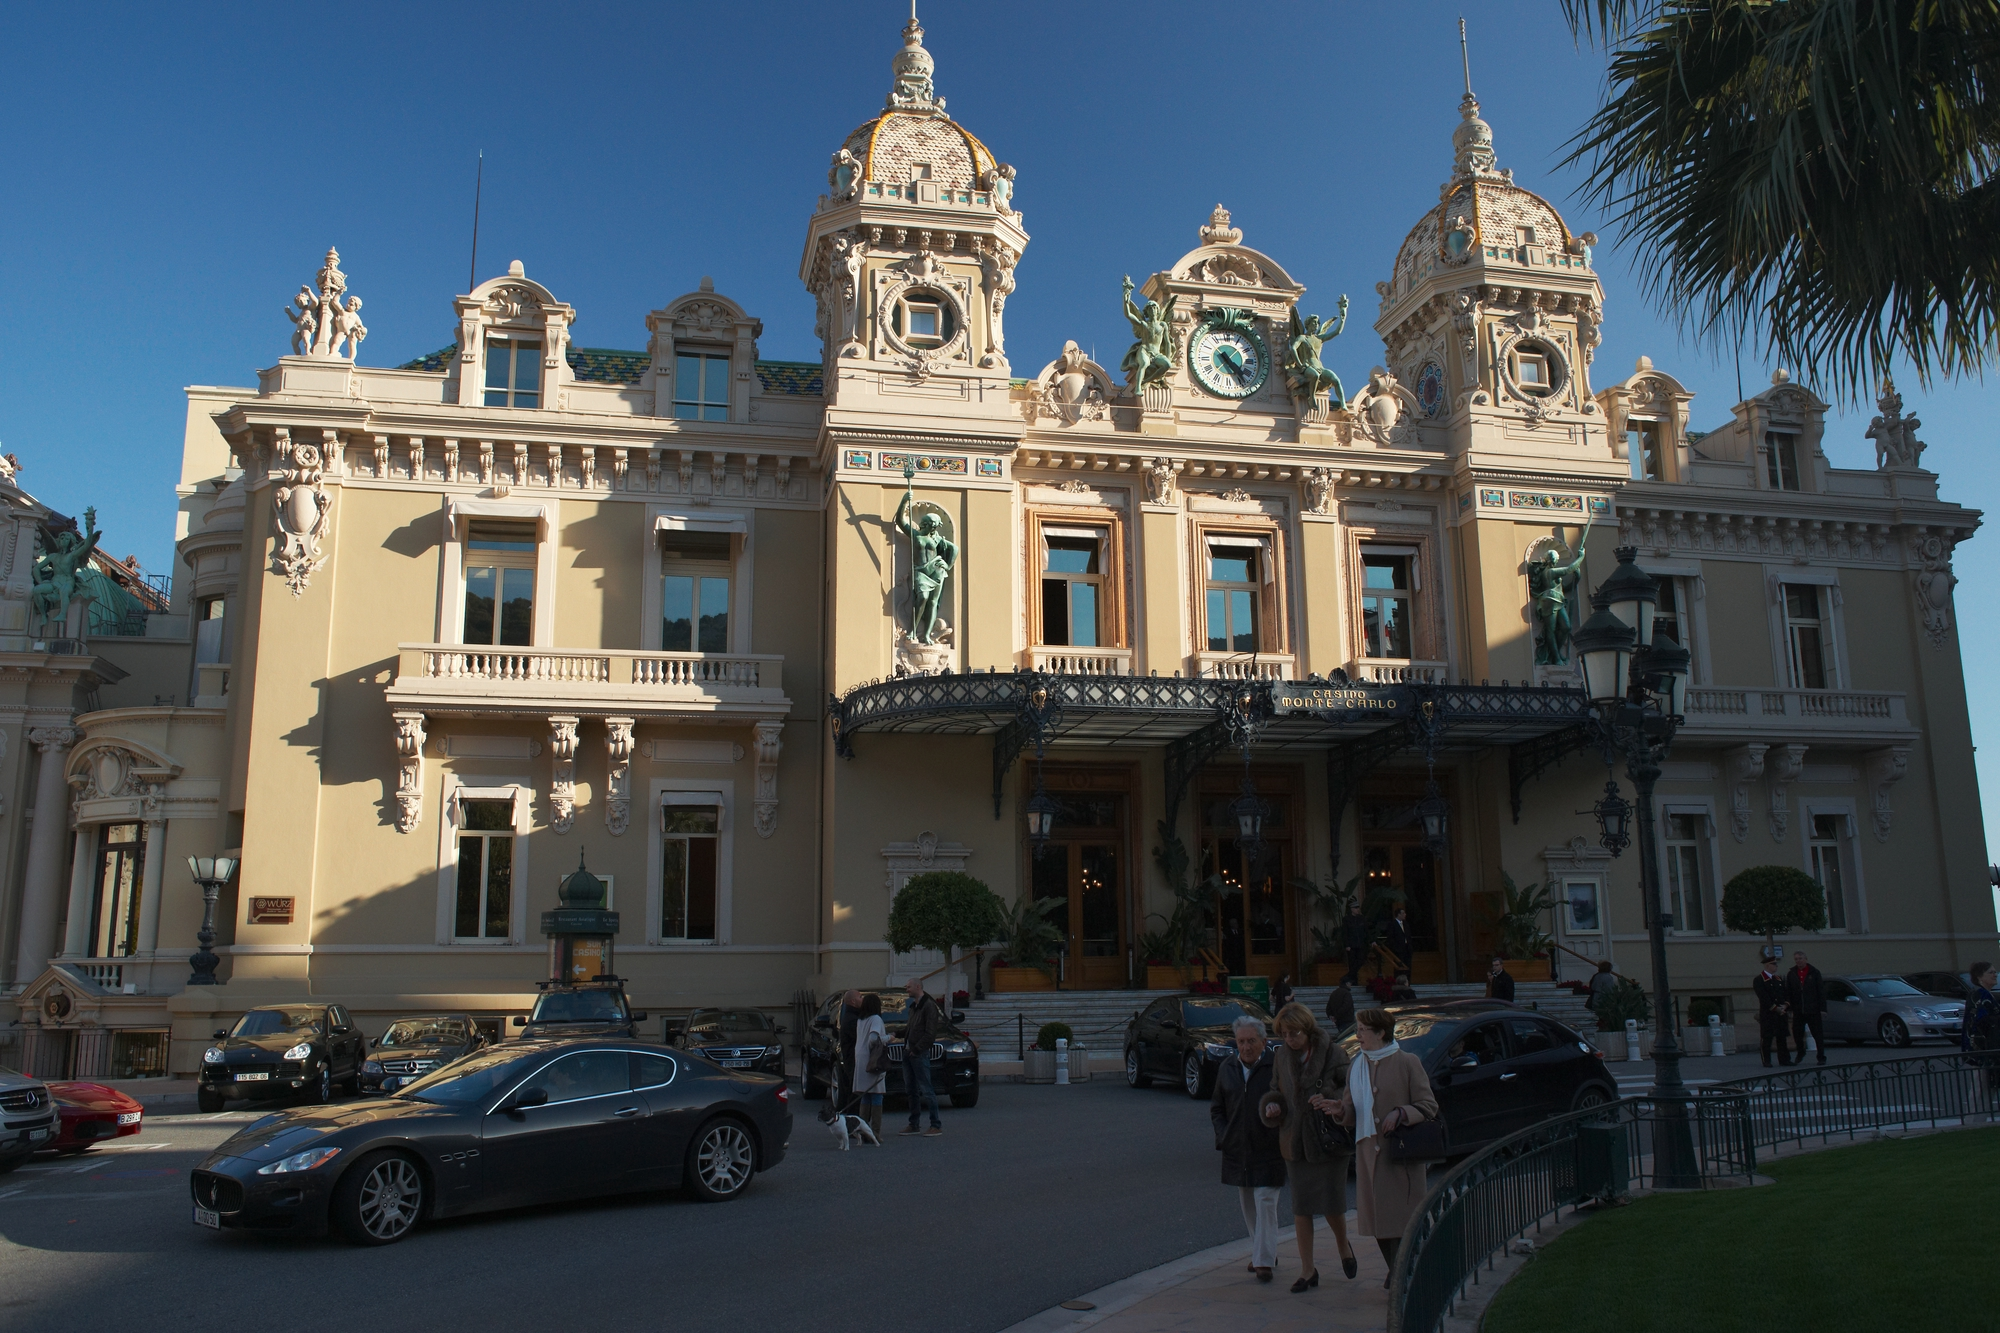
\includegraphics[width=0.7\textwidth]{images/monaco-02.jpg}}
\end{frame}

\subsection{Случайные величины}
\begin{frame}[fragile]
  \frametitle{Случайные величины}
  \begin{itemize}
    \item Своё название основной метод моделирования случайных процессов берёт от одного из округов княжества Монако, в котором издревле ``обитает'' огромное количество казино.
    \item ``Рулетка'' --- один из наиболее известных примеров ``относительно случайной'' величины. \footnote{Конечно, не в случае ``правильного'' крупье.}
    \item Другой пример случайной величины --- результат бросания монетки (орёл / решка).
    \item Или игрального кубика.
    \item В разных случаях количество вариантов может быть разным, но сохраняется принцип случайности (или \emph{псевдослучайности}).
  \end{itemize}
\end{frame}

\subsection{Случайные величины 2}
\begin{frame}[fragile]
  \frametitle{Случайные величины}
  \begin{itemize}
    \item Одно из основных свойств случайной величины --- строгое подчинение законам теории вероятности.
    \item К примеру, если мы 100 раз подбросим монетку, то примерно в 50 случаях выпадет орёл (50\%).
    \item Разумеется, в реальности будут \emph{промахи}. Например, 58 орлов (58\%).
    \item Однако чем больше \emph{испытаний}, тем ближе итоговый процент будет к вероятному.
    \item 8 ``лишних'' орлов на 1000 испытаний --- это уже не 8\%, а 0.8\%.
  \end{itemize}
\end{frame}

\subsection{Принцип}
\begin{frame}
  \begin{center}
    \Large{Чем выше количество испытаний, тем точнее результат}
  \end{center}
\end{frame}

\subsection{Вопрос}
\begin{frame}
  \begin{center}
    \Huge{Вопрос}
  \end{center}
  \begin{center}
    \Large{Если в рулетке я буду всё время ставить на красное, выиграю я, проиграю ли или же останусь ``при своих''?}
  \end{center}
\end{frame}

\section{Метод Монте-Карло}

\subsection{Метод Монте-Карло}
\begin{frame}[fragile]
  \frametitle{Метод Монте-Карло}
  \begin{itemize}
    \item Изначально прототип классического метода Монте--Карло был предложен Ферми и развит фон Нейманом для решения дифференциальных уравнений.
    \item Идея была развита Уламом, который, во время болезни раскладывая пасьянсы, решил подсчитать, с какой вероятностью пасьянс сложится.
    \item Вместо сложной комбинаторной задачи был предложен следующий метод: провести множество экспериментов со случайным набором карт и посчитать количество совпавших. Оно и даст некую приближенную величину к искомой.
    \item Появление компьютеров позволило проводить такое моделирование для большого количества испытаний, что и привело в 1949 году к возникновению метода Монте--Карло (казино).
  \end{itemize}
\end{frame}

\subsection{Примеры Монте-Карло}
\begin{frame}
  \begin{center}
    \Huge{Примеры использования метода Монте--Карло}
  \end{center}
\end{frame}

\subsection{Биология}
\begin{frame}
  \begin{center}
    \Huge{Биология}
  \end{center}
  \begin{center}
    \Large{Теория эволюции, генетика, вирусология, эпидемиология, \textbf{нейронные сети} и др.}
  \end{center}
\end{frame}

\subsection{Астрономия}
\begin{frame}
  \begin{center}
    \Huge{Астрономия}
  \end{center}
  \begin{center}
    \Large{Движение планет, астероидов, комет, свойства звёзд, галактик и Вселенной и др.}
  \end{center}
\end{frame}

\subsection{Физика}
\begin{frame}
  \begin{center}
    \Huge{Физика}
  \end{center}
  \begin{center}
    \Large{Метеорология, гидродинамика, нанотехнологии, ядерная физика\footnote{Водородная бомба} и др.}
  \end{center}
\end{frame}

\subsection{Экономика}
\begin{frame}
  \begin{center}
    \Huge{Экономика}
  \end{center}
  \begin{center}
    \Large{Бизнес-аналитика, финансовый анализ, технический анализ, экономическая теория и др.}
  \end{center}
\end{frame}

\subsection{Математика}
\begin{frame}
  \begin{center}
    \Huge{Математика}
  \end{center}
  \begin{center}
    \Large{Дифференциальные уравнения, интегрирование, математическая физика и др.}
  \end{center}
\end{frame}

\subsection{Апофис}
\begin{frame}[fragile]
  \frametitle{Пример вычислений}
  
  \centerline{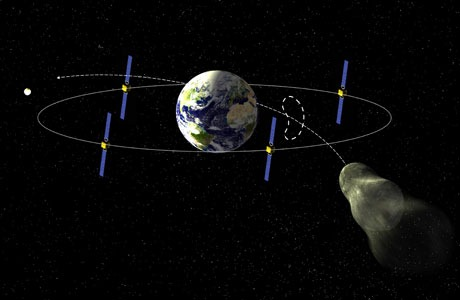
\includegraphics[width=0.5\textwidth]{images/apophis.jpg}}
  \begin{itemize}
    \item При прохождении астероида через указанную область в 2029 г. он обязательно врежется в 2036 г. 
    \item Сама область получена моделированием методом Монте--Карло.
  \end{itemize}
  
\end{frame}

\section{Реализация}

\subsection{Реализация}
\begin{frame}[fragile]
  \frametitle{Реализация в ruby}
  \begin{itemize}
    \item Прежде всего для метода Монте--Карло нужен генератор случайных чисел. 
    \item В ruby есть одна функция, которая умеет их генерировать. Она выдаёт разные результаты в зависимости от аргумента:
    \item
    \begin{tabular}{|c|c|}
      \hline
      Пример & Описание \\
      \hline
      rand() & возвращает случайное число от 0 до 1 \\
      \hline
      rand(5..20) & возвращает целое число от 0 до 19 \\
      \hline
    \end{tabular}
  \end{itemize}
\end{frame}

\subsection{Пример программы}
\begin{frame}[fragile]
  \frametitle{Пример использованиея}
  
  \begin{itemize}
    \item Выведем на экран случайное число от 0 до 9, от 0 до 135 и ещё одно от 1 до 100 и запишем последнее в переменную r.
  \end{itemize}
    \begin{lstlisting}[language=ruby,basicstyle=\footnotesize,label=ruby1,caption=Случайные числа]
      puts rand(10)
      puts rand(136)
      r = rand(100)+1
      puts r
    \end{lstlisting}
\end{frame}

\subsection{Пи}
\begin{frame}[fragile]
  \frametitle{Вычисление числа Пи}
  \begin{itemize}
    \item В качестве простого примера научимся вычислять число $\pi$.
  \end{itemize}
  \centerline{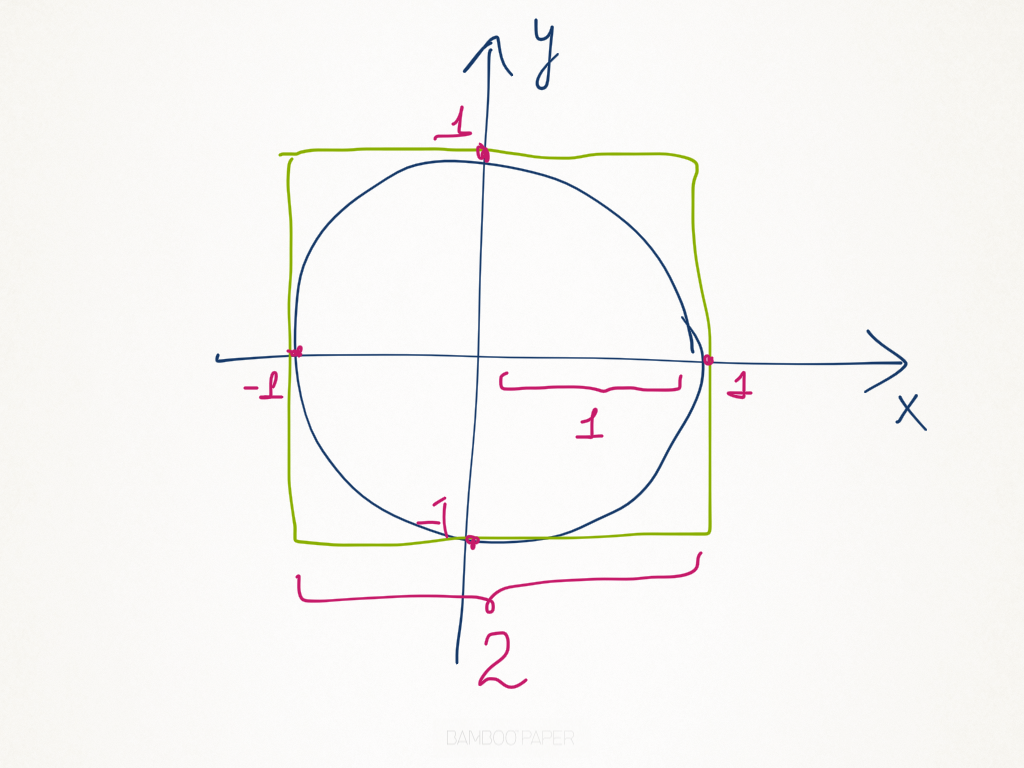
\includegraphics[width=0.7\textwidth]{images/pi-monte-carlo.png}}
\end{frame}

\subsection{Идея Пи}
\begin{frame}[fragile]
  \frametitle{Идея решения}
  \begin{itemize}
    \item Рассмотрим круг радиусом 1, расположенный в начале координат.
    \item Опишем вокруг круга квадрат стороной 2.
    \item Будем бросать в квадрат точки со случайными координатами.
    \item Вероятность $p$ попадания точки равна отношению площади круга $S_{circle}$ к площади квадрата $S_{square}$.
  \end{itemize}
\end{frame}

\subsection{Идея Пи 2}
\begin{frame}[fragile]
  \frametitle{Идея решения}
  \begin{itemize}
    \item $S_{circle} = \pi\cdot R^2 = \pi\cdot 1^2 = \pi$.
    \item $S_{square} = 2^2 = 4$
    \item $p = \cfrac{\pi}{4}$ => $\pi = 4\cdot p$.
    \item Как же понять, что точка $(x,y)$ лежит внутри круга? 
    \item Очень просто: $x^2 + y^2 < 1^2$.
    \item Итого, вычислив вероятность, найдём число $\pi$.
  \end{itemize}
\end{frame}

\subsection{Вычисление Пи}
\begin{frame}[fragile]
  \frametitle{Вычисление Пи}
    \scriptsize{
    \begin{lstlisting}[language=ruby,basicstyle=\footnotesize,label=ruby2,caption=Вычисление Пи]
      count=0
      n=1000
      n.times do |i|
        x = rand()
        y = rand()
        count+=1 if (x**2+y**2 < 1)
      end
      puts (count.to_f/n)*4
    \end{lstlisting}
    }
\end{frame}

\subsection{Результаты Пи}
\begin{frame}[fragile]
  \frametitle{Результаты}
  \begin{itemize}
    \item Проверим результат при разных $n$:
    \item
    \begin{tabular}{|l|l|}
      \hline
      n & $\pi$ \\
      \hline
      10 & 3.2 \\
      \hline
      100 & 3.04 \\
      \hline
      1000 & 3.156 \\
      \hline
      10000 & 3.1396 \\
      \hline
      100000 & 3.1448 \\
      \hline
      1000000 & 3.143 \\
      \hline
      10000000 & 3.1417 \\
      \hline
    \end{tabular}
  \end{itemize}
\end{frame}

\section{Парадоксы}
\subsection{Парадокс Монти-Холла}
\begin{frame}[fragile]
  \frametitle{Парадокс Монти-Холла}
  \begin{itemize}
    \item Представьте, что вы стали участником игры, в которой вам нужно выбрать одну из трех дверей. За одной из дверей находится автомобиль, за двумя другими дверями --- козы. Вы выбираете одну из дверей, например, номер 1, после этого ведущий, который знает, где находится автомобиль, а где --- козы, открывает одну из оставшихся дверей, например, номер 3, за которой находится коза. После этого он спрашивает вас, не желаете ли вы изменить свой выбор и выбрать дверь номер 2. Увеличатся ли ваши шансы выиграть автомобиль, если вы примете предложение ведущего и измените свой выбор?
  \end{itemize}
\end{frame}

\subsection{Дилемма заключённого}
\begin{frame}[fragile]
  \frametitle{Дилемма заключённого}
  \begin{itemize}
    \item Двое преступников, А и Б, попались примерно в одно и то же время на сходных преступлениях. Есть основания полагать, что они действовали по сговору, и полиция, изолировав их друг от друга, предлагает им одну и ту же сделку: если один свидетельствует против другого, а тот хранит молчание, то первый освобождается за помощь следствию, а второй получает максимальный срок лишения свободы (10 лет). Если оба молчат, их деяние проходит по более лёгкой статье, и они приговариваются к 6 месяцам. Если оба свидетельствуют против друг друга, они получают минимальный срок (по 2 года). Каждый заключённый выбирает, молчать или свидетельствовать против другого. Однако ни один из них не знает точно, что сделает другой. Что произойдёт?
  \end{itemize}
\end{frame}

\end{document}